\chapter{More on Tree}

\section{Tries}
\subsection{Definition}
A trie, also called a digital tree, radix tree, or prefix tree, is a special type of tree used to store associative data structures. The name trie comes from its use for re\textbf{trie}val, because the trie can find a single word in a dictionary with only a prefix of the word. 

\begin{minipage}{0.5\textwidth}
For example, strings are stored in a top-to-bottom manner based on their prefixes in a trie. All prefixes of length 1 are stored at level 1, all prefixes of length 2 are stored at level 2, and so on. For the string set \( S = \{ \text{bear}, \text{bell}, \text{bid}, \text{bull}, \text{but}, \text{sell}, \text{stock}, \text{stop} \} \), we can have the tree structure as shown on the right. \\[3pt]
This figure shows how the strings are stored in the trie. Inserting and deleting words in this tree is straightforward. For example, when typing "belt," it can be inserted in the subtree starting from \verb|b -> e -> l|. \\[3pt]
Unlike a binary search tree, no node in a trie stores the key associated with that node; instead, its position in the tree defines the key with which it is associated.
\end{minipage}
\begin{minipage}{0.5\textwidth}
\begin{figure}[H]
  \centering
  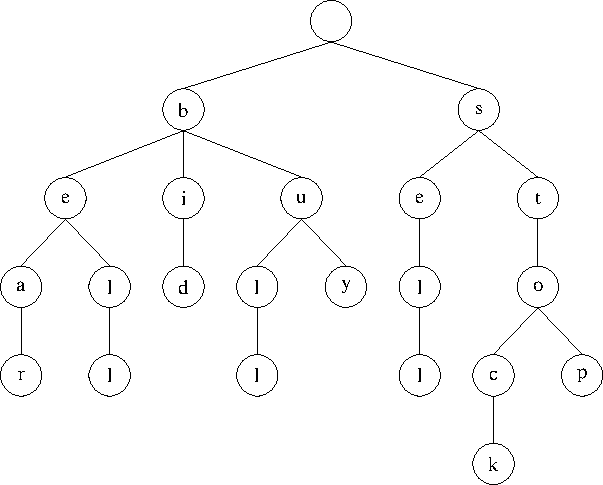
\includegraphics[width=0.8\textwidth]{Figure/Tries.pdf}
  \caption{Tries}
\end{figure}
\end{minipage}

 

All the descendants of a node share a common prefix in the string associated with that node, and the root is associated with the empty string.

\subsection{Applications}
A trie can also be used to replace a hash table, offering the following advantages:

1. Faster lookup: Looking up data in a trie is faster than the worst case of a hash table. For a trie, the time complexity is \(O(m)\), where \(m\) is the length of the search string. However, the time for an imperfect hash table would be \(O(n)\), where \(n\) is the total number of strings.

2. No collisions: There are no collisions of different keys in a trie, unlike hash tables, where collisions can occur when two keys map to the same hash value.

3. No need for a hash function: In a trie, there is no need to provide a hash function or change it as more keys are added, unlike hash tables that require such adjustments.

4. Alphabetical ordering: A trie can provide an alphabetical ordering of the entries by key, making it useful for applications like autocomplete or lexicographical ordering.

A common application of a trie is storing a predictive text or autocomplete dictionary, such as those found on mobile phones. It is also used in web browsers, which autocomplete your text or show possible completions for the text you are typing. Additionally, a trie can act as an orthographic corrector, checking whether every word you type exists in a dictionary.

\subsection{Analysis}
A standard trie uses \(O(n)\) space and supports searches, insertions, and deletions in time \(O(dm)\), where \(n\) is the total size of the strings in \(S\), \(m\) is the size of the string parameter of the operation, and \(d\) is the size of the alphabet.

\section{B-Tree}
Here we continue the discussion on B-Trees.  

A B-Tree is a self-balanced search tree with multiple keys in each node and can have more than two children per node. The properties of B-Trees have been discussed in the previous chapter.  

Following these properties, for example, a B-Tree of order 4 contains a maximum of 3 key values in a node and a maximum of 4 children for a node.  
\begin{figure}[H]
  \centering
  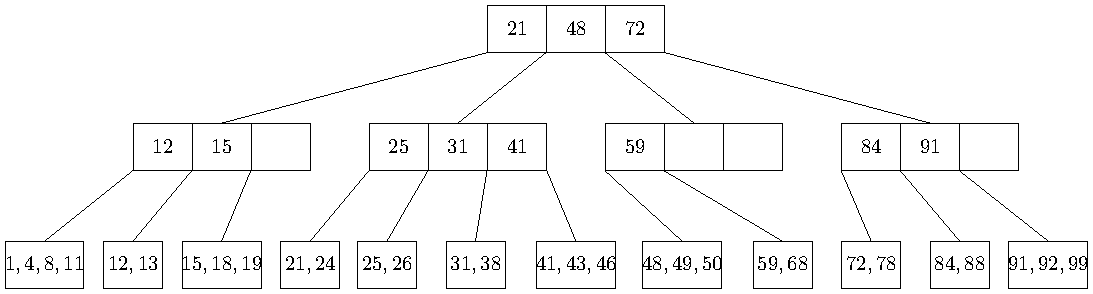
\includegraphics[width=\textwidth]{Figure/B-Tree.pdf}
  \caption{B-tree of order 4}
\end{figure}

\subsection{Operations}
To search for a certain element in a B-Tree, we first read the value from the user. Then, we compare the search element with the first key value of the root node in the tree. If they match, we terminate the function immediately. If they do not match, we check whether the search element is smaller or larger, then move to the appropriate subtree where the element could be found. This process is done recursively until we either find the exact match or complete the comparisons with the last key value in a leaf node.

In a B-Tree, a new element must be added only at a leaf node. This means new key values are always attached to leaf nodes.

To perform an insertion, we first check if the tree is empty. If it is empty, we create a node with the new key value and insert it into the tree as the root node. Otherwise, we find the appropriate leaf node where the new key value can be added, using binary search tree logic. If the leaf node has an empty position, we add the new key value to the leaf node, maintaining the ascending order of key values within the node.

If the leaf node is already full, we split that leaf node by sending the middle value to its parent, and repeat this process until the value is placed into a node. If the split reaches the root, the middle value becomes the new root node, increasing the height of the tree by one.

Following, we construct a B-Tree of order 3 by inserting numbers from 1 to 8.

\begin{center}
\begin{minipage}{0.1\textwidth}
\begin{figure}[H]
  \centering
  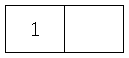
\includegraphics[width=\textwidth]{Figure/BT_D1.pdf}
\end{figure}
\end{minipage}\quad
\begin{minipage}{0.1\textwidth}
\begin{figure}[H]
  \centering
  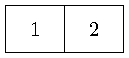
\includegraphics[width=\textwidth]{Figure/BT_D2.pdf}
\end{figure}
\end{minipage}\quad
\begin{minipage}{0.3\textwidth}
\begin{figure}[H]
  \centering
  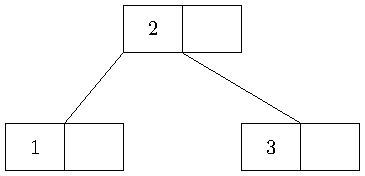
\includegraphics[width=\textwidth]{Figure/BT_D3.pdf}
\end{figure}
\end{minipage}\quad
\begin{minipage}{0.3\textwidth}
\begin{figure}[H]
  \centering
  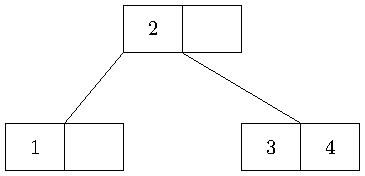
\includegraphics[width=\textwidth]{Figure/BT_D4.pdf}
\end{figure}
\end{minipage}
\end{center}

For 1 and 2, we can directly do the insertion. For 3, since the node is full, we split the node by sending the middle value 2 to the parent node. Since there is an empty position, we can directly insert 4.

\begin{center}
\begin{minipage}{0.4\textwidth}
\begin{figure}[H]
  \centering
  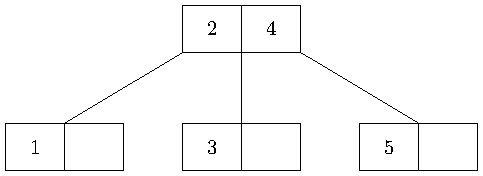
\includegraphics[width=\textwidth]{Figure/BT_D5.pdf}
\end{figure}
\end{minipage}\quad
\begin{minipage}{0.4\textwidth}
\begin{figure}[H]
  \centering
  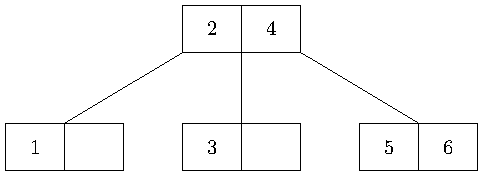
\includegraphics[width=\textwidth]{Figure/BT_D6.pdf}
\end{figure}
\end{minipage}
\end{center}

Since the rightmost node is full, we insert 5 by sending the middle value to the parent node and split the node. Then, we can directly insert 6.

\begin{center}
\begin{minipage}{0.45\textwidth}
\begin{figure}[H]
  \centering
  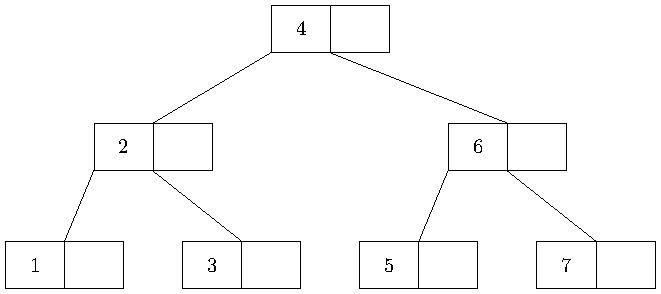
\includegraphics[width=\textwidth]{Figure/BT_D7.pdf}
\end{figure}
\end{minipage}
\begin{minipage}{0.45\textwidth}
\begin{figure}[H]
  \centering
  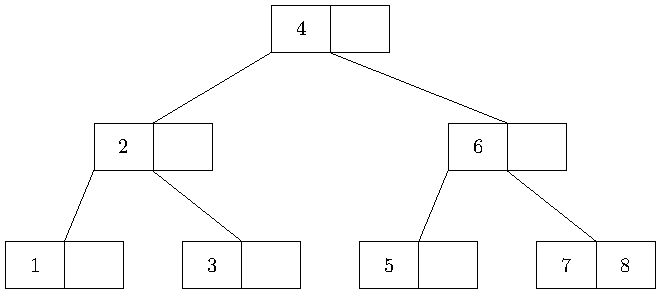
\includegraphics[width=\textwidth]{Figure/BT_D8.pdf}
\end{figure}
\end{minipage}  
\end{center}

Since the rightmost node is again full, we insert 7 by sending the middle value and splitting the node. Since the parent is also full, we further split it and send the middle value, in this case 4, to the parent node. To insert 8, it can be done directly.

To do deletion, if the key to be deleted is in a leaf and it contains more than the minimum number of keys, then this key can be deleted with no further action. If it is not a leaf, swap it with its successor under the natural order of the keys, then delete the key from the leaf. 

If the node contains the minimum number of keys, consider the two immediate siblings of the node. If one of these siblings has more than the minimum number of keys, then redistribute one key from this sibling to the parent node, and one key from the parent to the deficient node. This is a rotation that balances the nodes. 

If both immediate siblings have exactly the minimum number of keys, then merge the deficient node with one of the immediate sibling nodes and one key from the parent node. If this leaves the parent node with too few keys, then the process is propagated upward.

\subsection{Analysis}
The depth of a B-Tree is \(h\), then  
\[
  h \leq \log_t \frac{n + 1}{2}, \quad t = \left\lceil \frac{m}{2} \right\rceil, \quad n = \text{the number of keys}.  
\]
The search, insertion, and deletion time is \(O(t \log_t n)\).
